% Generated by scripts/build_slides.py from saved results.
\documentclass[aspectratio=169,11pt]{beamer}
\usepackage[T1]{fontenc}
\usepackage{lmodern}
\usepackage{graphicx}
\usepackage{booktabs}
\definecolor{banner}{HTML}{1B3A6B}
\definecolor{accent}{HTML}{2E6DB4}
\setbeamercolor{frametitle}{bg=banner,fg=white}
\setbeamercolor{title}{fg=banner}
\setbeamercolor{structure}{fg=banner}
\setbeamercolor{item}{fg=accent}
\setbeamertemplate{navigation symbols}{}
\setbeamertemplate{footline}[frame number]
\newcommand{\slide}[1]{\begin{frame}[plain]\makebox[\textwidth]{\includegraphics[width=\paperwidth]{figures/#1}}\end{frame}}

\title{When Trading Dries Up}
\subtitle{A liquidity signal for a long-only fund}
\author{Group 7 \\ Silver Fund}
\date{Built on 2011--2018, tested on held-back 2019--2024}

\begin{document}
\begin{frame}\titlepage\end{frame}

\begin{frame}{The idea}
\begin{itemize}
\item A \textbf{liquidity event}: a stock suddenly trades far less than usual for it (measured against its own past year).
\item \textbf{Why it should matter:} most investors avoid illiquid stocks; only a small group of patient investors holds them, at a slightly lower price.
\item When a stock's trading collapses, it has to pass from its current holders to that small group.
  \begin{itemize}
  \item Sellers can only exit slowly, because volume has dried up; the few buyers need a lower price.
  \item So the price \textbf{walks down for months}. Shorting these stocks is costly, so nobody trades the drift away.
  \end{itemize}
\item We first remove anything the fund's six existing scores already capture.
\item Questions: is the effect real, and can our long-only fund make money from it?
\end{itemize}
\end{frame}

\begin{frame}{Bottom line}
\begin{itemize}
\item \textbf{Yes, it is real.} Stocks whose trading dries up keep falling: about 3\% behind similar stocks over the next year.
\item \textbf{Just avoiding them doesn't help:} +0.05\% to +0.10\% a year, not significant.
\item \textbf{Betting against them daily with the optimizer works}, also on 2019--24 data we held back: long-only +0.51\% a year (IR 1.05).
\item \textbf{It is small:} about +0.31\% a year after trading costs. Use it as one input to the fund's alpha.
\end{itemize}
\end{frame}

\slide{matched_drift.png}
\slide{where.png}

\begin{frame}{It is not something we already know}
\centering
\small
\begin{tabular}{lr}
\toprule
 & How much less flagged stocks earn, \%/month ($t$) \\
\midrule
Had a liquidity event in the last month & 0.18 (2.5) \\
... also controlling for last month's return & 0.17 (2.4) \\
\bottomrule
\end{tabular}

\medskip
\raggedright\footnotesize Positive = flagged stocks earn less, which is what we bet on. Monthly regressions of next month's return, 2008--2018; every row also controls
for size, how illiquid the stock already was, its past-year return and its return two to three years ago, and the fund's six scores were removed before flagging.
Measured once a month, so it understates the first-weeks effect that daily trading captures.
\end{frame}

\begin{frame}{The simple idea doesn't work: just avoid these stocks}
\centering
\small
\resizebox{\linewidth}{!}{%
\begin{tabular}{lrrrrr}
\toprule
2011--2018 & Weight avoided & Return & Risk & IR ($t$) & IR, market removed \\
\midrule
Just avoid flagged stocks, daily & 8.6\% & +0.05\%/yr & 0.47\% & 0.11 (0.3) & $-$0.12 \\
Just avoid flagged stocks, monthly & 8.7\% & +0.10\%/yr & 0.43\% & 0.23 (0.7) & $-$0.12 \\
\midrule
Optimizer, daily, no shorting & --- &+0.19\%/yr & 0.10\% & 1.82 (5.1) & --- \\
\bottomrule
\end{tabular}}

\medskip
\raggedright\footnotesize
\begin{itemize}
\item Hold the benchmark, sell every stock with a liquidity event in the last 63 days, give its weight to similar stocks.
\item It barely earns anything: these stocks are small, so dropping them tilts the portfolio in ways that add noise and swamp the effect.
\item The optimizer removes that noise and sizes each bet. That is what makes the signal pay.
\end{itemize}
\end{frame}

\begin{frame}{How we bet on it}
\begin{itemize}
\item \textbf{Alpha} (Grinold--Kahn, Manual 4.6): $\alpha_i = IC \times \sigma_i \times Z_i$.
  \begin{itemize}
  \item Our $Z_i$ is a flag: did stock $i$ have a liquidity event 1--21 days ago, or 22--63 days ago?
  \item We estimate $IC \times Z$ directly: the average gap to similar stocks per unit of volatility, for each age (a regression on a 0/1 flag, Manual 4.4). Past years only, re-estimated every January.
  \end{itemize}
\item \textbf{Optimizer} (Manual ch.\ 3): maximize $h^\top\alpha - \tfrac{\gamma}{2} h^\top V h$ with $h^\top\iota = 0$, $h^\top\beta = 0$, 5\% tracking error, and size and liquidity in line with the benchmark.
\item \textbf{Two versions:} no limits, and no shorting ($b + h \ge 0$, Manual 3.4). The transfer coefficient extends the fundamental law to $IR = TC \times IC \sqrt{BR}$: TC is how much of the forecast survives the long-only rule.
\item \textbf{No trading costs:} the signal would be one input to the fund's alpha, where trades net out. We show what it would cost alone.
\end{itemize}
\end{frame}

\slide{vol_check.png}

\begin{frame}{Daily rebalancing, 2011--2018 and holdout 2019--2024}
\begin{columns}[T]
\begin{column}{0.50\textwidth}
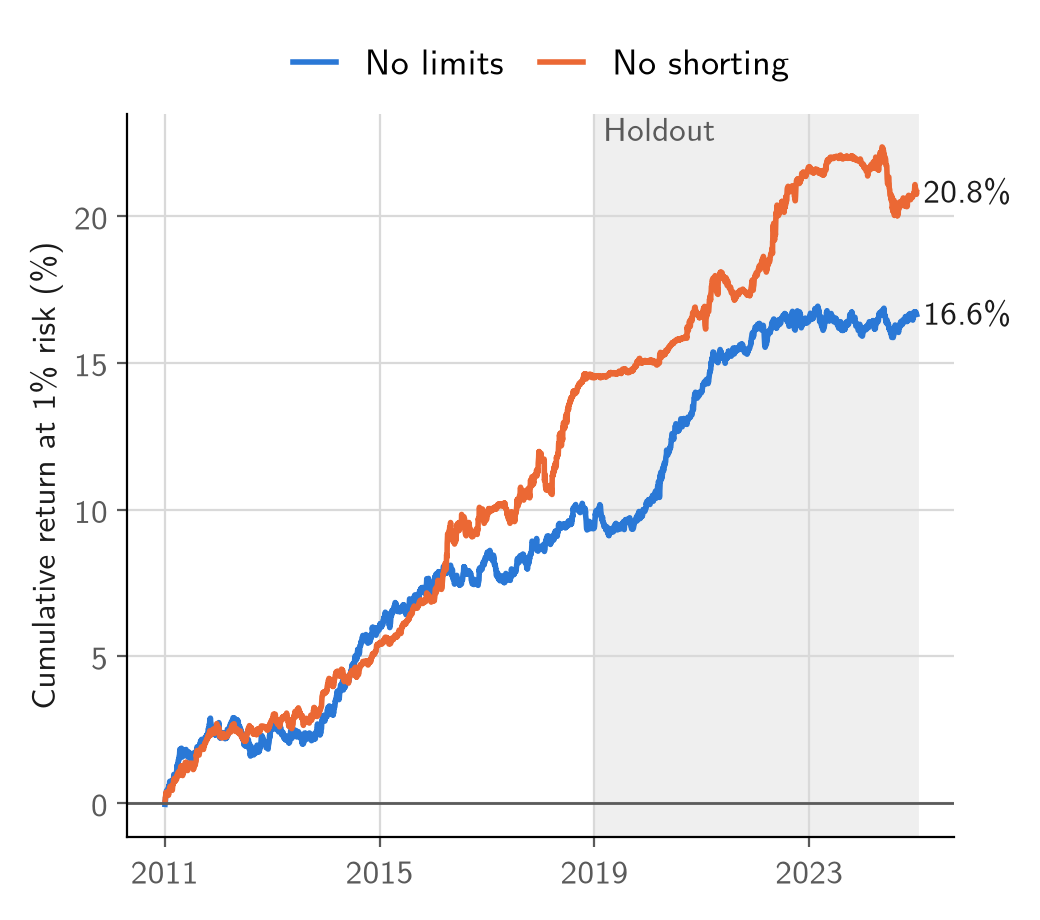
\includegraphics[width=\linewidth]{figures/pair_daily.png}
\end{column}
\begin{column}{0.48\textwidth}
\vspace{10mm}
\scriptsize
\resizebox{\linewidth}{!}{%
\begin{tabular}{lrrrr}
\toprule
 & \multicolumn{2}{c}{No limits} & \multicolumn{2}{c}{No shorting} \\
\cmidrule(lr){2-3}\cmidrule(lr){4-5}
 & 2011--18 & 2019--24 & 2011--18 & 2019--24 \\
\midrule
Active return, \%/yr & +6.84 & +7.43 & +0.19 & +0.51 \\
Active risk (realized) & 5.82\% & 6.12\% & 0.10\% & 0.48\% \\
IR ($t$) & 1.17 (3.3) & 1.21 (3.0) & 1.82 (5.1) & 1.05 (2.6) \\
Max drawdown & $-$7.62\% & $-$6.53\% & $-$0.15\% & $-$1.14\% \\
Positive years & 7/8 & 5/6 & 8/8 & 5/6 \\
Turnover, $\times$/yr & 186.4 & 166.9 & 2.2 & 4.5 \\
TC vs no limits & ref. & ref. & 0.44 & 0.36 \\
Spread cost if traded alone, \%/yr & 14.06 & 15.91 & 0.09 & 0.19 \\
\bottomrule
\end{tabular}}
\end{column}
\end{columns}
\vspace{1mm}
{\scriptsize Each period's line scaled to 1\% realized risk; the table shows actual numbers. No shorting = total weight $\ge 0$.
TC = ex-ante transfer coefficient vs.\ no limits. Holdout: design frozen before it was run; settings re-estimated each January from earlier years only.\par}
\end{frame}

\begin{frame}{Monthly rebalancing, 2011--2018 and holdout 2019--2024}
\begin{columns}[T]
\begin{column}{0.50\textwidth}
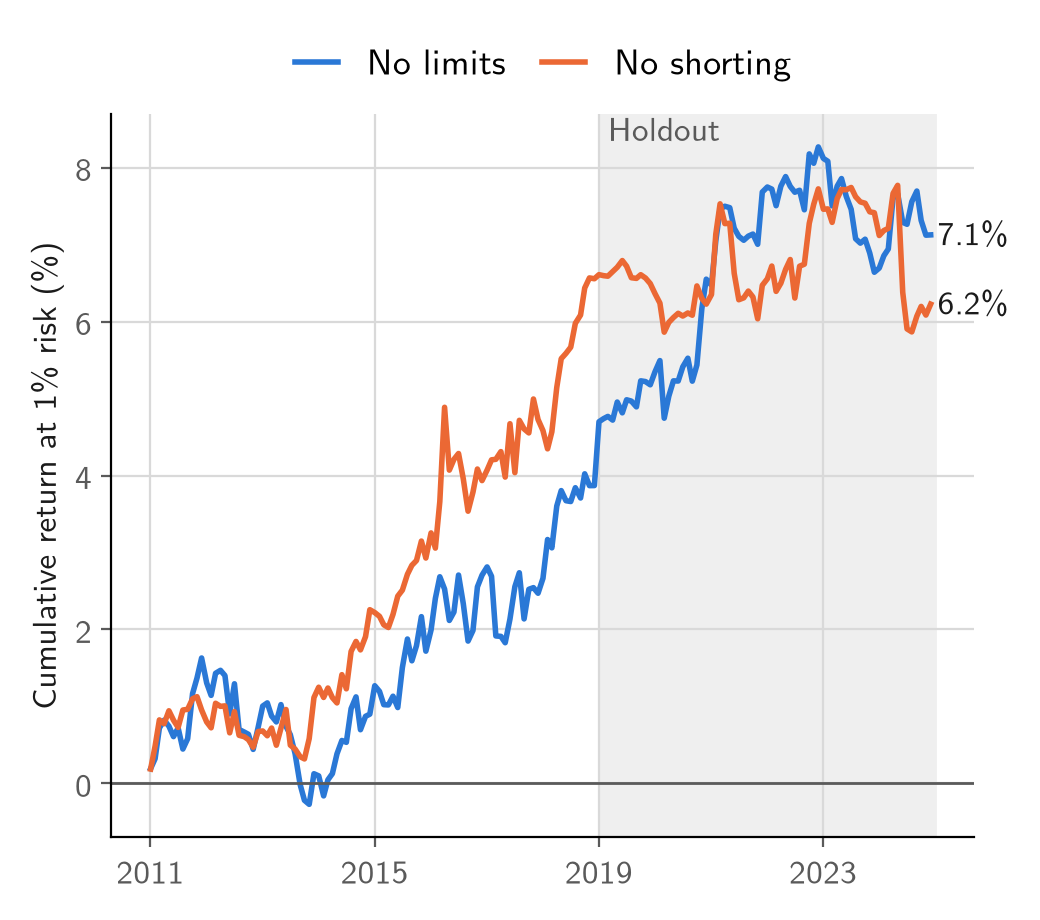
\includegraphics[width=\linewidth]{figures/pair_monthly.png}
\end{column}
\begin{column}{0.48\textwidth}
\vspace{10mm}
\scriptsize
\resizebox{\linewidth}{!}{%
\begin{tabular}{lrrrr}
\toprule
 & \multicolumn{2}{c}{No limits} & \multicolumn{2}{c}{No shorting} \\
\cmidrule(lr){2-3}\cmidrule(lr){4-5}
 & 2011--18 & 2019--24 & 2011--18 & 2019--24 \\
\midrule
Active return, \%/yr & +2.92 & +3.58 & +0.08 & $-$0.02 \\
Active risk (realized) & 6.03\% & 6.59\% & 0.10\% & 0.44\% \\
IR ($t$) & 0.48 (1.4) & 0.54 (1.3) & 0.82 (2.3) & $-$0.05 ($-$0.1) \\
Max drawdown & $-$11.47\% & $-$10.74\% & $-$0.14\% & $-$0.84\% \\
Positive years & 5/8 & 5/6 & 7/8 & 2/6 \\
Turnover, $\times$/yr & 60.9 & 53.9 & 0.7 & 1.5 \\
TC vs no limits & ref. & ref. & 0.44 & 0.36 \\
Spread cost if traded alone, \%/yr & 5.63 & 6.28 & 0.02 & 0.05 \\
\bottomrule
\end{tabular}}
\end{column}
\end{columns}
\vspace{1mm}
{\scriptsize Each period's line scaled to 1\% realized risk; the table shows actual numbers. No shorting = total weight $\ge 0$.
TC = ex-ante transfer coefficient vs.\ no limits. Holdout: design frozen before it was run; settings re-estimated each January from earlier years only.\par}
\end{frame}

\begin{frame}{How much to trust it}
\begin{itemize}
\item We built it on 2011--18 in four rounds, then froze it and ran 2019--24 \textbf{once}.
\item In 2019--24 the long-only portfolio is bigger (0.48\% risk vs 0.10\%): the model learned that large stocks drift too, so it had more weight to sell (appendix).
\item After trading costs, long-only earns about +0.31\% a year (IR about 0.6).
\item Six years is short (standard error of an IR $\approx 1/\sqrt{\text{years}}$): the true IR could be anywhere from about 0.2 to 1.9.
\end{itemize}
\end{frame}

\begin{frame}{Conclusion}
\begin{itemize}
\item Stocks whose trading dries up keep falling for months: they must pass to a small group of patient buyers, and that hand-off is slow.
\item A long-only fund can make money from it, but only with the optimizer and daily trading.
\item It is small. Use it as one input to the fund's alpha, not on its own.
\item Next: combine it with the fund's scores and test the combined alpha, with trading costs.
\end{itemize}
\end{frame}

\begin{frame}[plain]\vfill\centering{\Large\textbf{\color{banner}Appendix}}\vfill\end{frame}

\slide{ic_by_year.png}

\begin{frame}{Appendix: what did we change, and when?}
\centering
\scriptsize
\begin{tabular}{lrr}
\toprule
Daily runs, \%/yr (IR), no costs & No limits & No shorting \\
\midrule
1. Flag that turns over daily & $-0.9$ ($-0.15$) & --- \\
2. Event clock & $-$2.77 ($-$0.49) & $-$0.12 ($-$0.24) \\
3. + no positive alpha, hedge with similar stocks & +3.23 (0.58) & +0.36 (1.48) \\
4. + alpha scaled by volatility & +6.84 (1.17) & +0.19 (1.82) \\
\bottomrule
\end{tabular}

\medskip
\raggedright\footnotesize
\begin{itemize}
\item Version 2: a flag that switched off after a few days missed most of the drift, so we gave each event an age.
\item Version 3: a noisy positive alpha for large stocks made the portfolio buy them; we stopped allowing positive alpha and hedged with similar stocks.
\item Version 4: calm stocks fell less than predicted (slide 9), so alpha now scales with volatility. Frozen before the 2019--24 test.
\end{itemize}
\end{frame}

\begin{frame}{Appendix: why is the long-only result bigger in 2019--24?}
\begin{columns}[T]
\begin{column}{0.48\textwidth}
\centering
\scriptsize
\resizebox{\linewidth}{!}{%
\begin{tabular}{lrrr}
\toprule
 & Large-stock & Long-only & Long-only \\
Year & alpha & risk & return \\
\midrule
2011 & 0.0 & 0.08\% & +0.25\% \\
2012 & 0.0 & 0.06\% & +0.04\% \\
2013 & 0.0 & 0.08\% & +0.10\% \\
2014 & $-$0.1 & 0.07\% & +0.17\% \\
2015 & 0.0 & 0.05\% & +0.16\% \\
2016 & $-$0.8 & 0.15\% & +0.28\% \\
2017 & $-$2.1 & 0.12\% & +0.21\% \\
2018 & $-$3.2 & 0.16\% & +0.29\% \\
\midrule \multicolumn{4}{l}{\textit{Holdout}} \\
2019 & $-$4.9 & 0.16\% & +0.26\% \\
2020 & $-$5.0 & 0.30\% & +0.76\% \\
2021 & $-$7.2 & 0.59\% & +0.63\% \\
2022 & $-$7.1 & 0.68\% & +1.80\% \\
2023 & $-$7.3 & 0.21\% & +0.06\% \\
2024 & $-$7.4 & 0.66\% & $-$0.47\% \\
\bottomrule
\end{tabular}}
\end{column}
\begin{column}{0.48\textwidth}
\footnotesize
\begin{itemize}
\item Until 2015 the model gave large stocks no alpha, so it could only sell small stocks, which hold little benchmark weight.
\item As evidence built up, large stocks got a negative alpha too, so the portfolio had more weight to sell.
\item Same signal, bigger portfolio.
\end{itemize}
\vspace{2mm}
\scriptsize Large-stock alpha: predicted daily drift per unit of volatility, $\times$10,000, for the first month after an event. Long-only: daily, no shorting.
\end{column}
\end{columns}
\end{frame}

\begin{frame}{Appendix: where does the return come from? (2011--2018)}
\centering
\small
\begin{tabular}{lrrr}
\toprule
Return, \%/yr & Event 1--21 days ago & Event 22--504 days ago & No recent event \\
\midrule
Daily, no limits & +14.88 & $-$3.43 & $-$4.64 \\
Daily, no shorting & +0.12 & +0.08 & $-$0.01 \\
Monthly, no limits & +8.02 & +0.09 & $-$4.09 \\
Monthly, no shorting & +0.09 & +0.06 & $-$0.05 \\
\bottomrule
\end{tabular}

\medskip
\raggedright\footnotesize Return earned on positions in stocks with a recent event, an older event, or none. In the no-limits runs the bets against flagged stocks are hedged
with similar stocks; small, illiquid stocks lag in general, so both sides show it and it cancels.
\end{frame}
\end{document}
